\section{The SM Higgs Boson}
\label{sec:smhiggs}

The introduction of a complex scalar field into the Standard Model 
to generate masses for the SM particles results in the prediction 
of a new massive scalar boson, 
the Higgs boson~\citep{Higgs:1964ia,PhysRev.155.1554,Higgs:1964pj,Guralnik:1964eu,PhysRev.145.1156}. 
The discovery of such a particle would give strong evidence as to the 
nature of electroweak symmetry breaking and hence many searches for it have been
launched since its existence was first proposed.

The mass of the SM Higgs boson, $\mh$, is not a predicted quantity in the SM
but is rather a function of the self-coupling parameter, $\lambda$, and 
$v$. The latter is determined experimentally to be $v=246$ GeV by precisely 
measuring the rate of muon decay~\citep{muondecay}.
However, since $\lambda$ is unconstrained, a large range in $\mh$ remains 
theoretically acceptable for the Higgs boson mass.

\subsection{Constraints and Previous Searches}

Several theoretical considerations constrain the mass of the SM Higgs 
boson~\citep{ellisHiggsReview}.
The desire to avoid the need for non-pertubative calculations for electroweak 
processes at high energies constrains the SM
Higgs boson mass to be less than around 770 GeV~\citep{higgstriviality}. 
Conversely, if $\mh$ is too small,
then the Higgs potential of Equation~\ref{eqn:higgslagr} contains a  
global minimum at large values of the scalar field $\phi$. Additional
physics, beyond that of the SM, would be required so that this global minimum
corresponds to the observed vacuum with $v=246$ GeV. 
This places a loose lower bound on the SM Higgs boson mass of about 115 
GeV~\cite{higgsreview2012}. 

\subsubsection{Direct Searches}
% LEP SENTENCE
The first direct constraints on the Higgs boson at higher masses 
were provided by the four experiments operating at the 
Large Electron-Positron (LEP) collider. By steadily increasing the centre of mass 
energy of the collisions, LEP was able to exclude masses of $m_{H} <114.4$ GeV at the 
95\% confidence level~\cite{lephiggs}. Prior to the LHC turn on, 
the CDF and D0 experiments at the Tevatron collider
provided additional limits on the mass of the Higgs boson through direct 
searches in proton anti-proton collisions. 
The centre of mass energy available in these collisions, $\sqrt{s}=1.96$ TeV, 
provided sensitivity to Higgs boson masses between 90 and 190 GeV. 
Priority at the Tevatron experiments was given to the $\Hww$ channel at high mass
and $\Hbb$, with associated production of a $W$ or $Z$ boson, at low mass.
By the shutdown of the Tevatron in 2011, the two experiments had collected combined 
datasets corresponding to a total integrated luminosity of $10fb^{-1}$. 
Figure~\ref{fig:tevatronlims} shows the 95\% confidence upper limits on the 
ratio of the excluded Higgs boson production cross-section to that predicted 
by the Standard Model as a function of $\mh$ obtained from this dataset. 
Mass hypotheses in the ranges $100\le\mh\le119 $ GeV and $141 \le \mh \le 184$ GeV
are excluded at the 95\% confidence level~\citep{tevhiggscombinations}.
\begin{figure}
\begin{center}
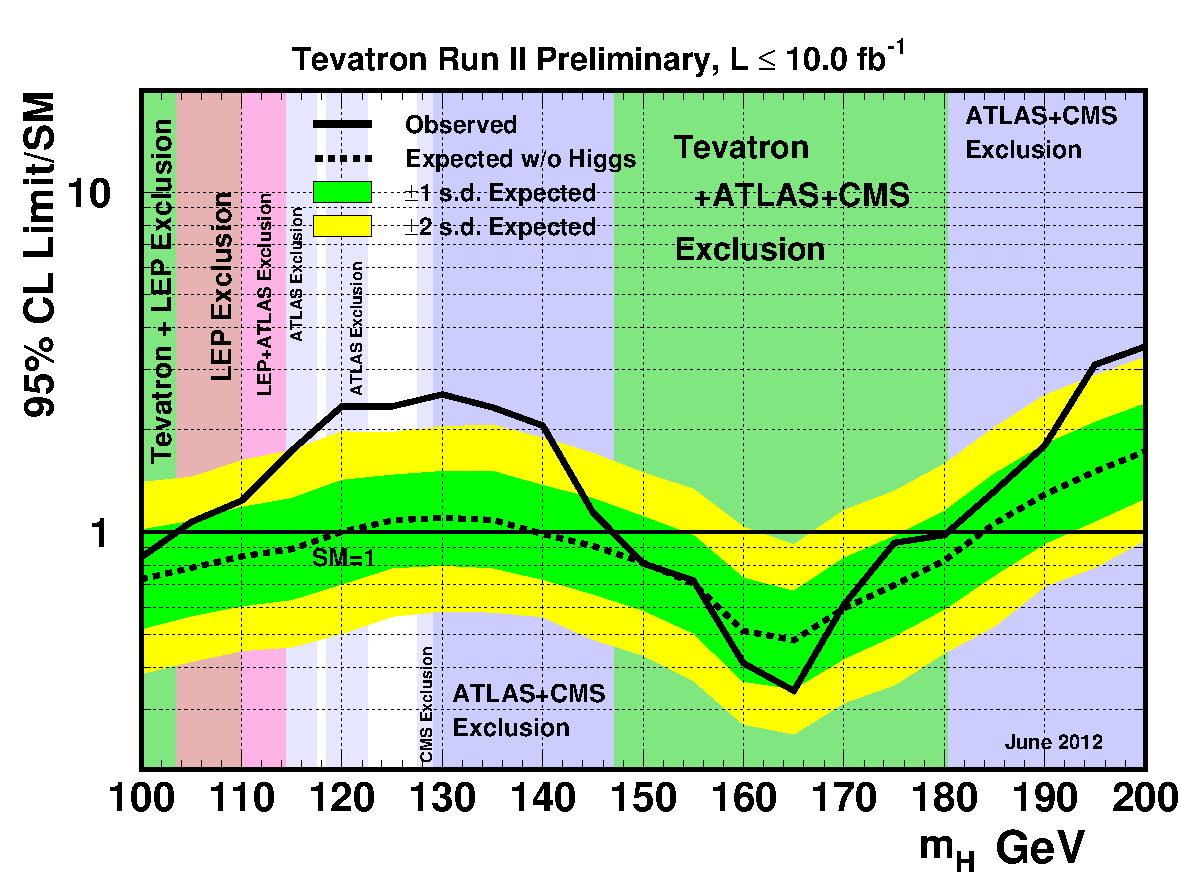
\includegraphics[width=0.8\textwidth]{theory/pheno/tevsmbayes_june2012_withleplhc.pdf}
\caption{The 95\% confidence upper limits on the ratio of Higgs boson production to the SM prediction
as a function of $\mh$.
The dotted line indicates the median expected exclusion assuming no
SM Higgs boson exists while the solid line indicates the observed exclusion obtained 
from the data. Where this line falls below 1, a SM Higgs boson with that mass is excluded at the
95\% confidence level as indicated by the green bands. The other coloured bands indicate 
exclusion limits resulting from direct searches for the SM Higgs boson conducted by other
Collaborations before June 2012. The figure has been altered from its original 
source~\cite{tevhiggscombinations}.}
\label{fig:tevatronlims}
\end{center}
\end{figure}

\subsubsection{Precision Measurements}
Collision data taken at the Tevatron are combined with precision measurements 
of electroweak observables performed at LEP
and by the SLD Collaboration based at SLAC to constrain the mass of the 
Higgs boson. Figure~\ref{fig:blueband} shows the relative chi-squared from a fit
to these data as a function of $\mh$. The minimum of the curve is at 94 GeV
with an experimental uncertainty of +29 and -24 GeV. The theoretical uncertainty
is indicated by the blue band. The yellow bands indicate the excluded regions in 
$\mh$ provided by direct searches for the SM Higgs boson conducted at LEP
and the LHC by March 2012.
\begin{figure}
\begin{center}
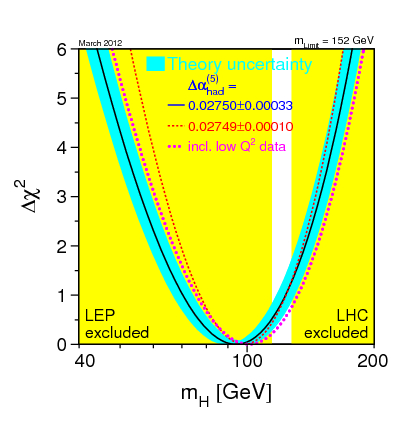
\includegraphics[width=0.6\textwidth]{theory/pheno/w12_blueband.jpg}
\caption{Delta chi-squared from global fit to combined data from CDF, D0, SLD and the LEP
Collaborations as a function of $\mh$~\cite{lepewwgpage}. 
The solid line is the nominal fit with theoretical
uncertainties indicated in blue while the dashed lines indicate alternative theoretical 
prescriptions. The yellow bands indicate the regions excluded at the 95\% confidence level
from direct searches for the SM Higgs boson conducted at LEP and the LHC before March 2012.} 
\label{fig:blueband}
\end{center}
\end{figure}

\subsection{Higgs Boson Production and Decay at the LHC}

At the LHC, protons are accelerated to higher energies than previously available at the 
Tevatron. The increased centre-of-mass energy enhances the 
rate at which Higgs boson production occurs and improves the sensitivity to higher 
masses. The four main mechanisms by which a Higgs boson can be produced
are shown at leading order in Figure~\ref{fig:higgsprodfeyn}.
\begin{figure}[hbtp!]
\begin{center}
%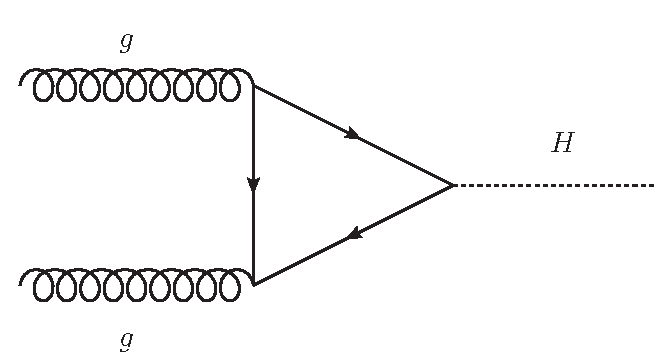
\includegraphics[width=.49\textwidth]{theory/pheno/ggh.pdf}
%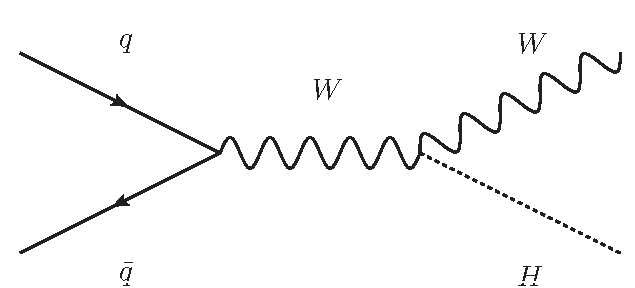
\includegraphics[width=.49\textwidth]{theory/pheno/vh.pdf}\\
%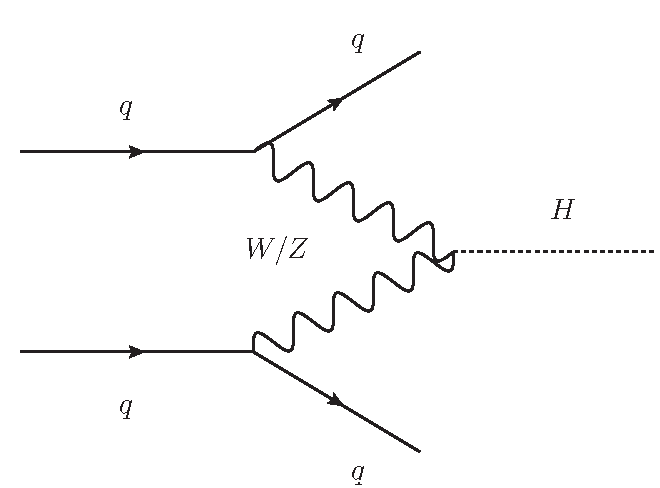
\includegraphics[width=.49\textwidth]{theory/pheno/qqh.pdf}
%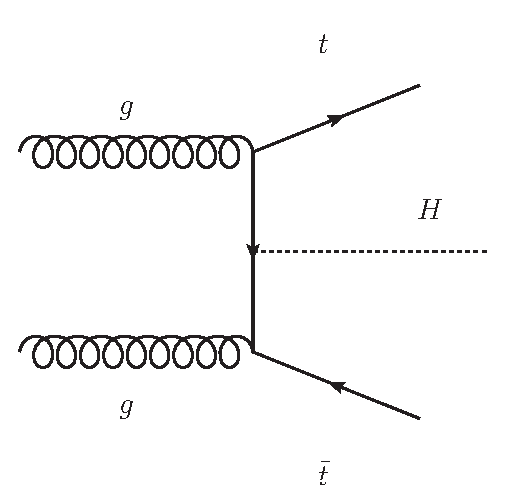
\includegraphics[width=.4\textwidth]{theory/pheno/tth.pdf}
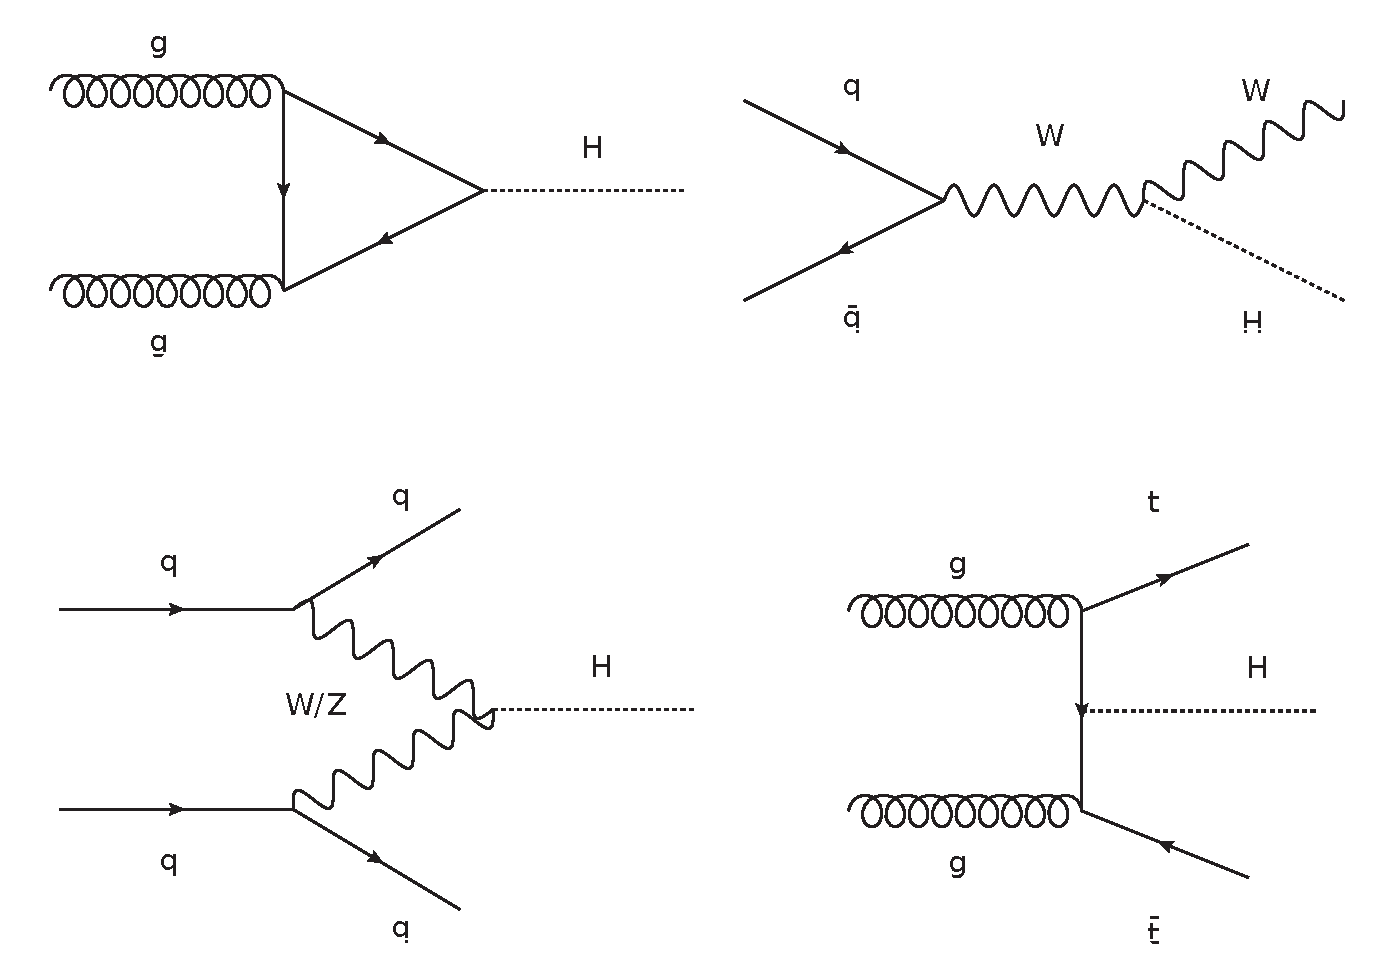
\includegraphics[width=\textwidth]{theory/pheno/allprods_new.pdf}
\caption{Dominant SM Higgs boson production mechanisms: Gluon-gluon fusion (top left),
vector-boson fusion (bottom left), associated production with vector boson (top right) 
and top anti-top quark pair (bottom right).}
\label{fig:higgsprodfeyn}
\end{center}
\end{figure}
The dominant production mechanism is through gluon-gluon fusion ($ggH$). As the gluons
are massless particles, the gluons couple to the Higgs boson via a quark-loop.
The three other production mechanisms which dominate Higgs boson production are 
vector boson fusion ($qqH$) and production in association with 
a $W$ or $Z$ boson ($VH$) or top anti-top quark pair ($ttH$).
Although these modes are at least an order of magnitude smaller in cross-section
than gluon-gluon fusion, their specific topologies 
can be exploited experimentally to enhance the signal over background processes 
(see Chapter~\ref{chap:combinations}).
Figure~\ref{fig:higgsprod} shows the production cross-sections and their theoretical 
errors for the four main production modes of the SM Higgs boson in  
p-p collisions at the LHC~\citep{lhcxswg2011,lhcxswg2012}.
\begin{figure}[hbtp!]
\begin{center}
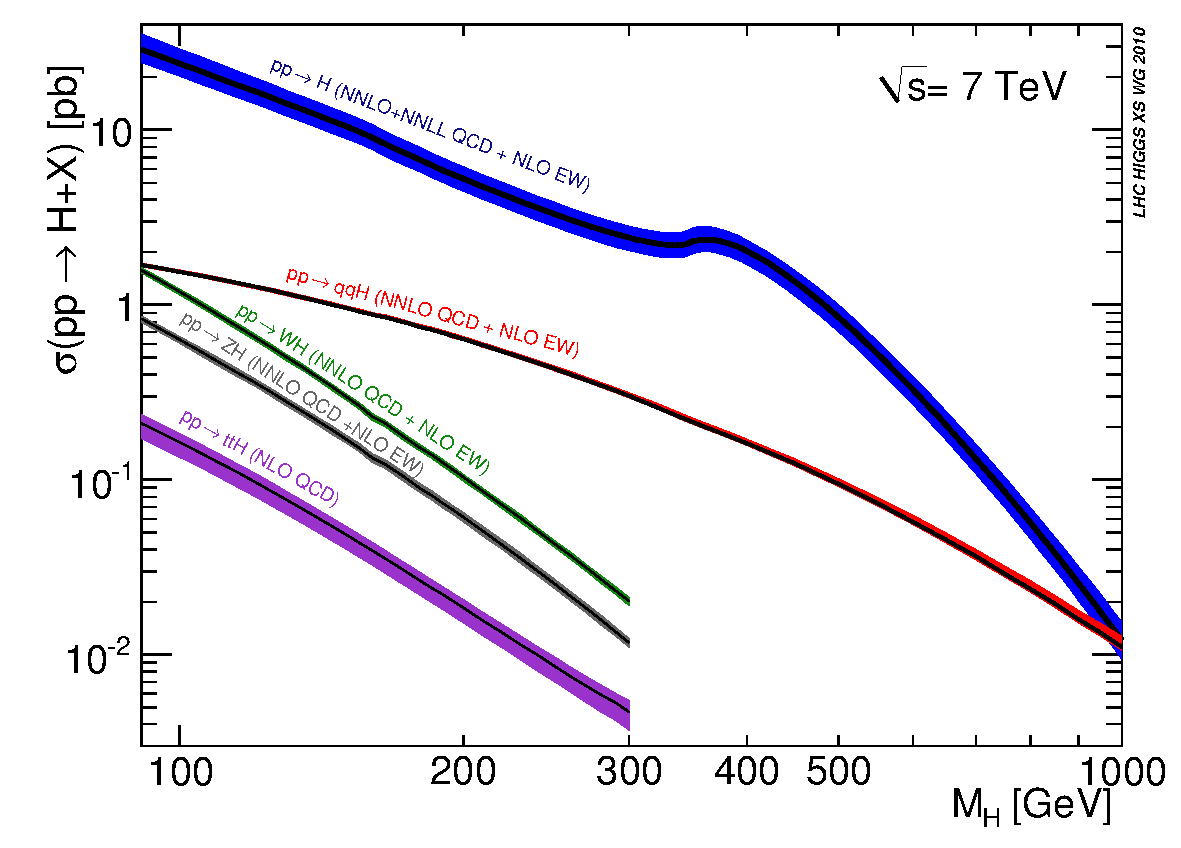
\includegraphics[width=0.8\textwidth]{theory/pheno/Higgs_XS_7TeV.pdf}\\
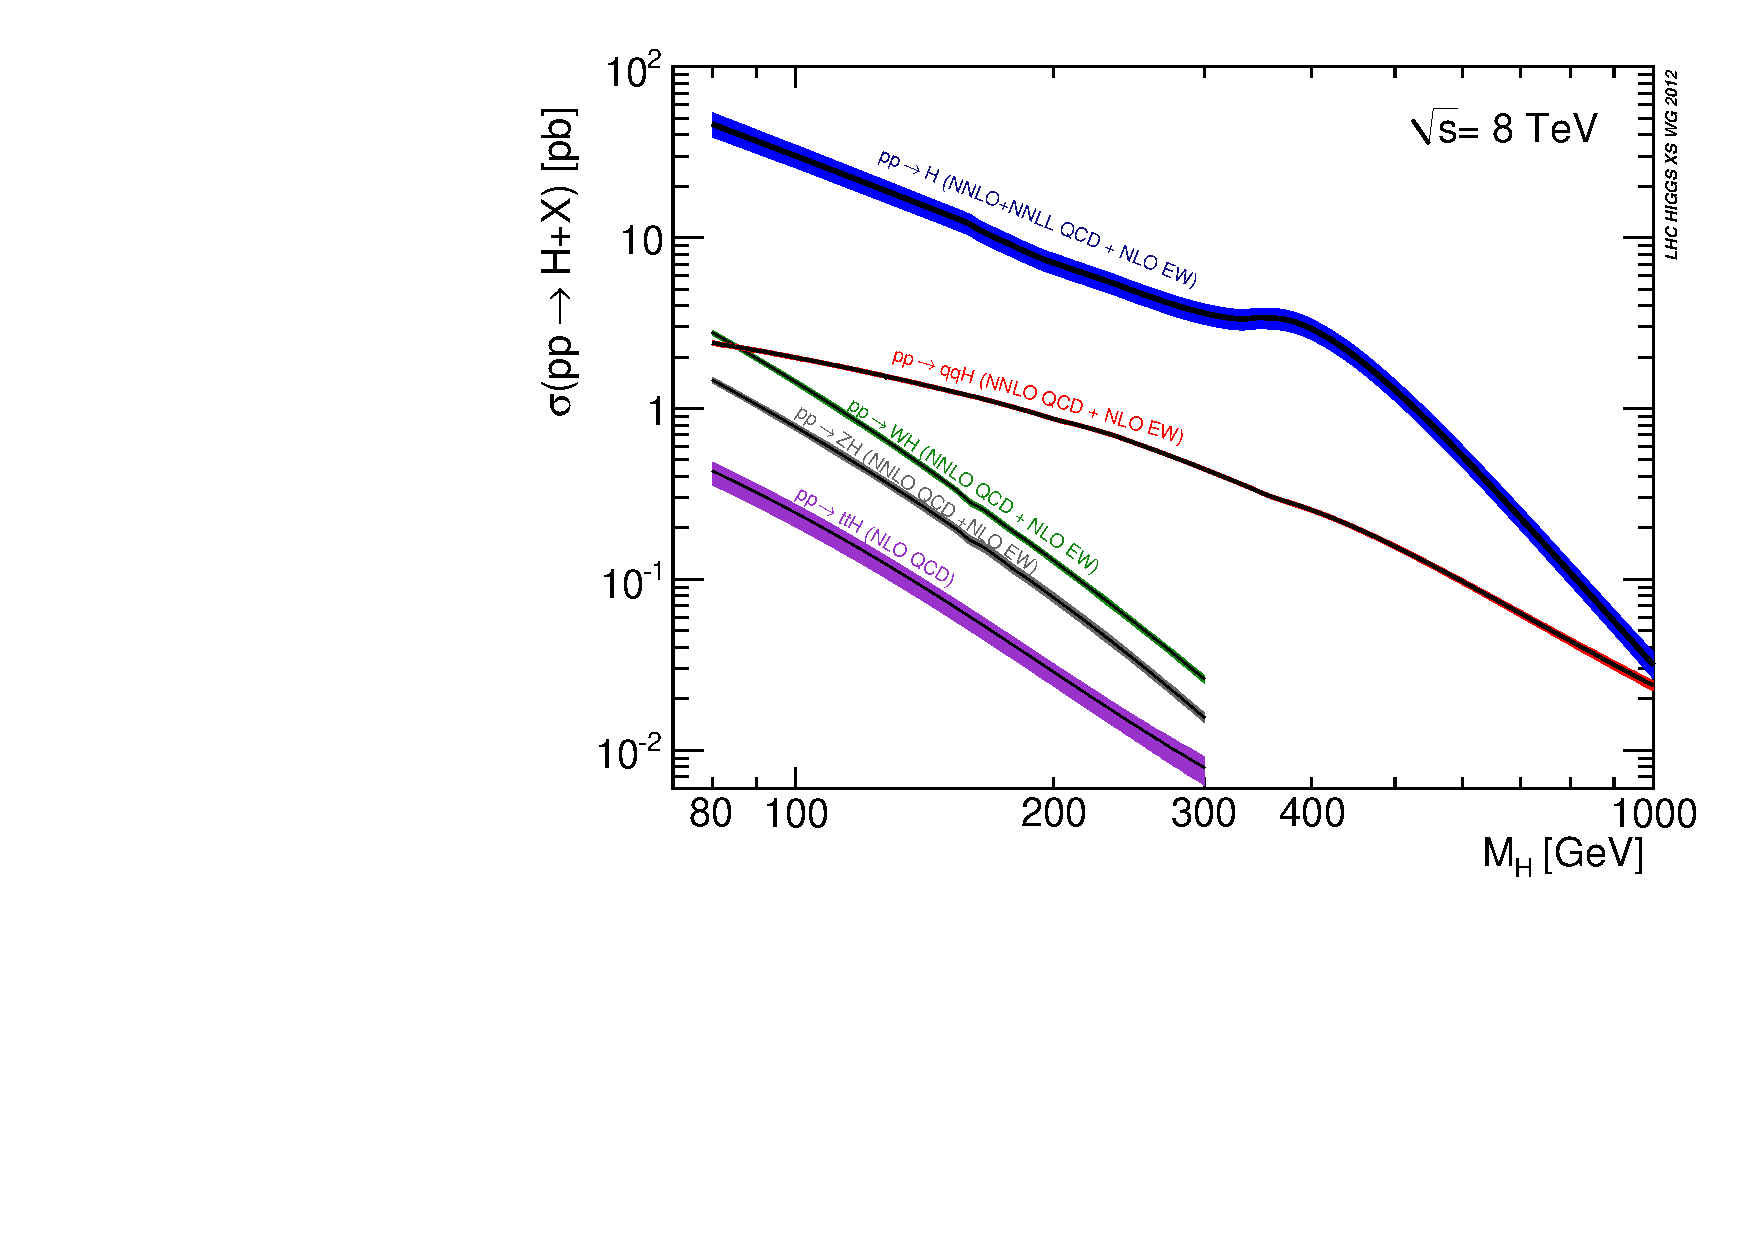
\includegraphics[width=0.8\textwidth]{theory/pheno/Higgs_XS_8TeV_lx.pdf}
\caption{SM Higgs boson production cross-sections at $\sqrt{s}=7~\mathrm{TeV}$ (top)
and 8 TeV (bottom) of the four main production mechanisms, $pp\rightarrow H+X$,
along with their theoretical uncertainties as a function of 
$\mh$~\citep{lhcxswg2011,lhcxswg2012}. The coloured bands indicate the theoretical
uncertainties.}
\label{fig:higgsprod}
\end{center}
\end{figure}
The Higgs boson is an unstable particle so will be observable directly at the LHC
only through its decay products. The relative decay rates (branching ratios) to 
different SM particles vary as a function of the Higgs boson mass.
At low mass, $\mh<135$ GeV, Higgs boson decay to a $b$ anti-$b$ quark pair
dominates. In proton-proton collisions, pairs of $b$-quarks are produced 
frequently making the background levels too high to compete with for an experimental
search. For higher masses, $\mh>180$ GeV, the Higgs boson is heavy enough
to facilitate production of real $W$ and $Z$ bosons which dominate its decay.
As the gluon and photon are massless, they do not directly couple to the Higgs boson
hence these decays are mediated by virtual loops of massive particles.
The branching ratios of the Higgs boson to SM particles are shown as a function
of $\mh$ in Figure~\ref{fig:higgsdecay} (left).

For small $\mh$, the natural width of the SM Higgs boson, $\hwidth$, is several
orders of magnitude smaller than its mass. Figure~\ref{fig:higgsdecay} (right) shows the 
value of the SM Higgs boson total width as a function of its mass.
This means that for decays in which the products are fully reconstructible in particle
detectors, the width of the invariant mass spectrum of the decay products will depend almost entirely
on the experimental resolution. 
In particular the ATLAS and CMS detectors provide excellent energy and momentum resolution 
for electrons, muons and photons.
Despite having lower branching ratios,  the $\Hgg$ and $\Hzzl$ channels
are therefore of particular importance for direct detection of the SM Higgs boson
at the LHC.


\begin{figure}[hbtp]
\begin{center}
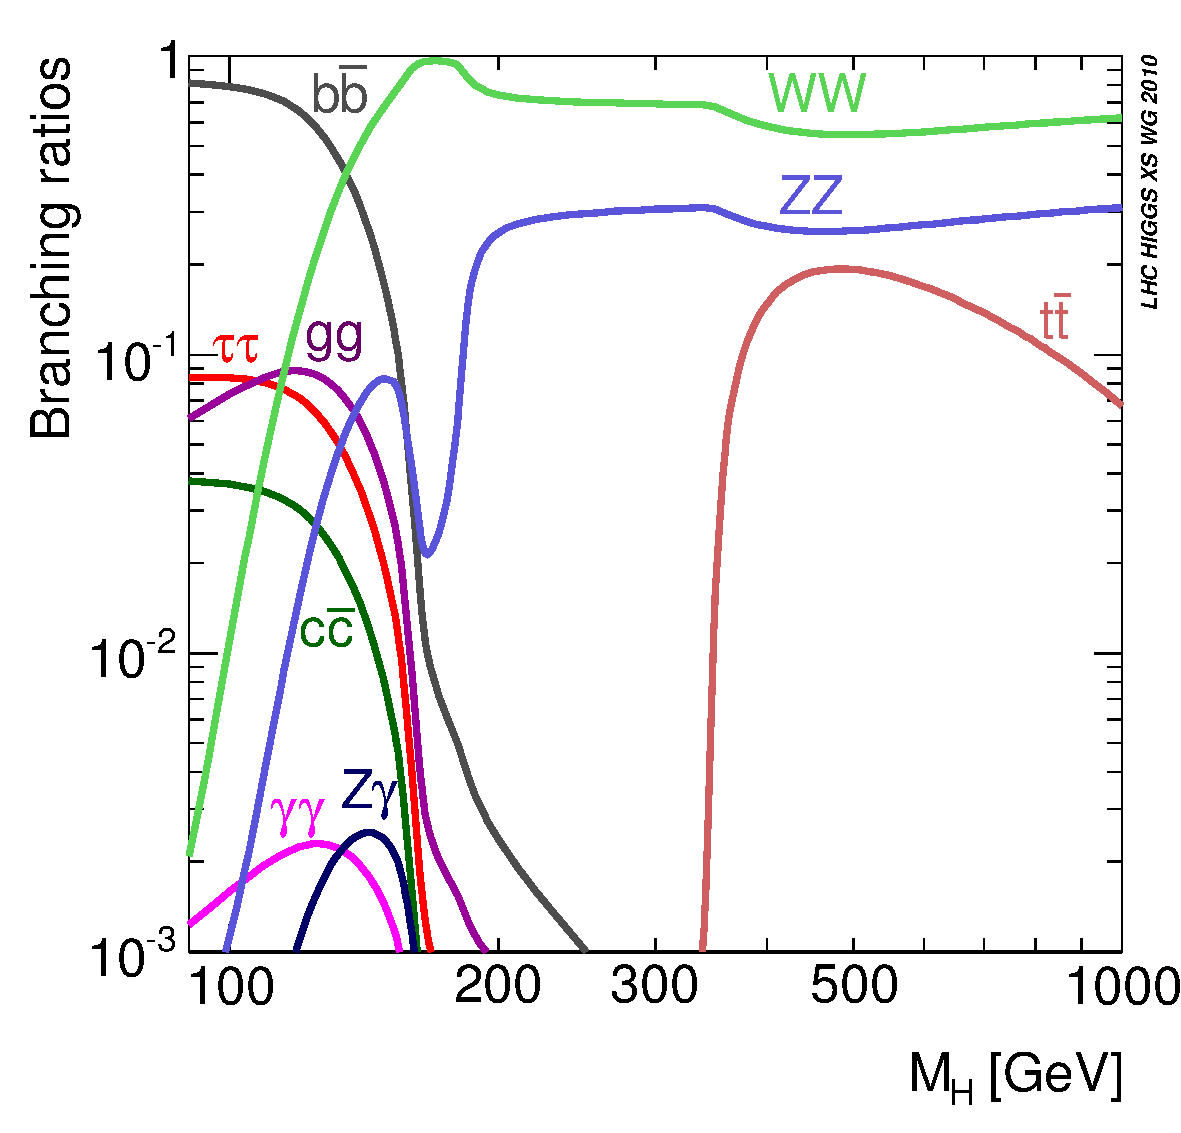
\includegraphics[width=0.49\textwidth]{theory/pheno/YRHXS_BR_fig3.pdf}
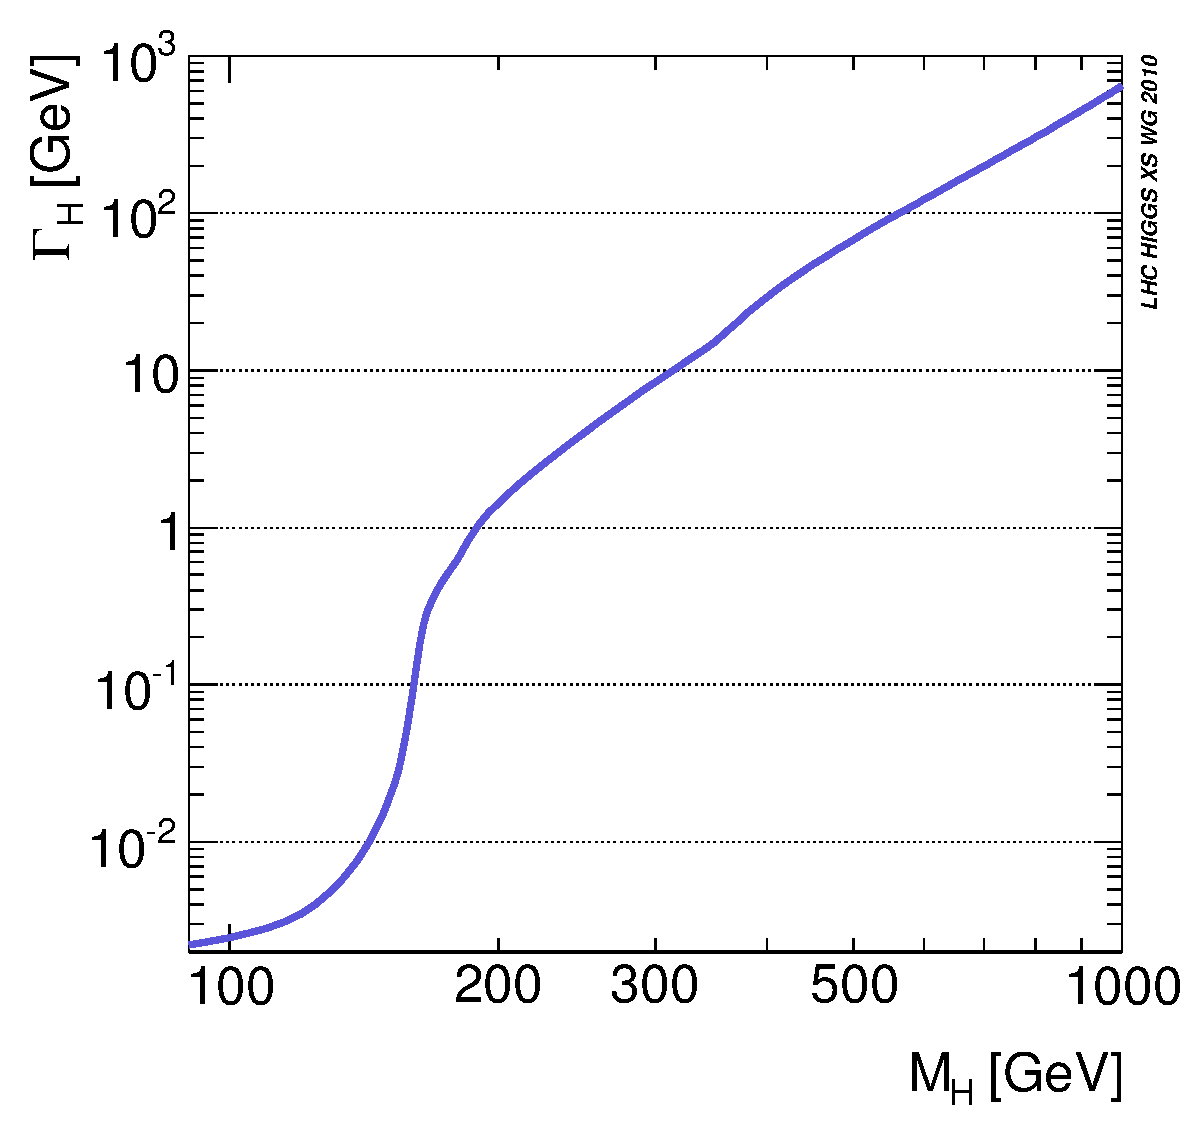
\includegraphics[width=0.49\textwidth]{theory/pheno/YRHXS_BR_fig2.pdf}
\caption{Left: SM Higgs boson production branching ratios for 
the dominant decays as a function of $\mh$. Right: SM Higgs boson total width, $\hwidth$, as 
a function of $\mh$~\citep{lhcxswg2011}.}
\label{fig:higgsdecay}
\end{center}
\end{figure}

